


\section{Introduction}
In perovskite solar cells, the absorber is usually sandwiched between two different contacts: the \gls{htm} and the \gls{etm}, with the role of extracting respectively the positive and negative free charges.
Without this asymmetrical extraction of charges, the photogeneration would be of no use.
The classical \gls{etm} from \gls{dssc}, mesoporous titania, is getting obsoleted by planar tin oxide \cite{Jiang2018}.
On the contrary, the classical \gls{htm} from solid-state \gls{dssc}, \gls{spiro}, is still present in most of the record structures of \gls{csfamapbibr} based solar cells \cite{Saliba2016,Saliba2018}.
The huge explorative work done for finding a better performing \gls{htm} managed to find very few good alternatives.% small molecules or polymers (\textsl{e.g.} \gls{ptaa}).
Still, even if the performances are at par with \gls{spiro}, the commercial price of these alternative \gls{htm} is still too high for wide area applications.
A better understanding of the \gls{htm}\-/perovskite interaction is needed for pinpointing the key characteristics to be looked for in the next \gls{htm} design.
In this chapter, the devices fabricated using four different \gls{htm}, have been compared in order to find a correlation with the \gls{htm}'s chemical properties.
Specifically we looked for the influence of the \gls{htm} on the device \gls{voc}.
Some authors observed a weak correlation between the \gls{htm} ionization potential and the cell voltage \cite{Polander2014,Abate2015a} while others suggested a complex interplay of factors where the \gls{htm} \gls{homo} just plays a marginal role \cite{Correa-Baena2017,Belisle2016,Ishida2016,Park2018,Jimenez-Lopez2017}.
The tested \gls{htm} were: the classic \gls{spiro}, the previously reported \gls{tae1} (CAS 1802982-22-4, after the first report in \cite{Cabau2015a}, it has been used also by other research groups in \cite{Choi2015b,Labban2016,Wu2016a,Wu2016b}) and two novel molecules: \glsdesc{tae3} (\gls{tae3}, CAS 2055756-83-5) and \glsdesc{tae4} (\gls{tae4}).

\begin{figure}
	\makebox[\textwidth][c]{
		\parbox{1.1\textwidth}{
			\centering
			\begin{subfigure}[t]{0.51\textwidth}
								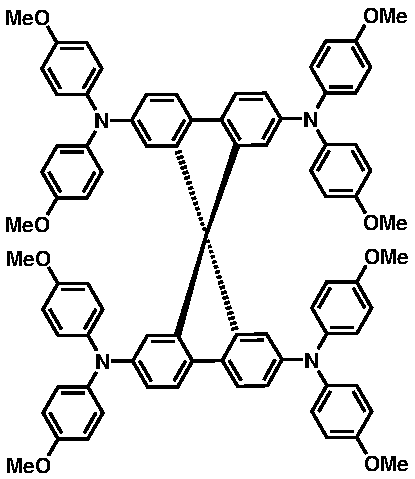
\includegraphics[scale=0.8]{molecules/spiro.pdf}
				\subcaption{\gls{spiro}}\label{fig:tae-molecules-spiro}
			\end{subfigure}
			\qquad
			\begin{subfigure}[t]{0.51\textwidth}
								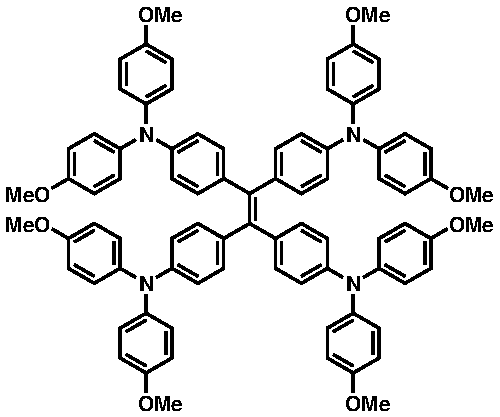
\includegraphics[scale=0.8]{molecules/tae1.pdf}
				\subcaption{\gls{tae1}}\label{fig:tae-molecules-tae1}
			\end{subfigure}
			\bigskip
			
			\begin{subfigure}[t]{0.51\textwidth}
				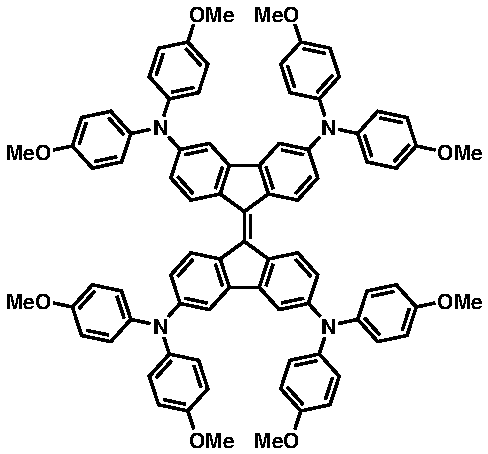
\includegraphics[scale=0.8]{molecules/tae3.pdf}
				\subcaption{\gls{tae3}}\label{fig:tae-molecules-tae3}
			\end{subfigure}
			\qquad
			\begin{subfigure}[t]{0.51\textwidth}
				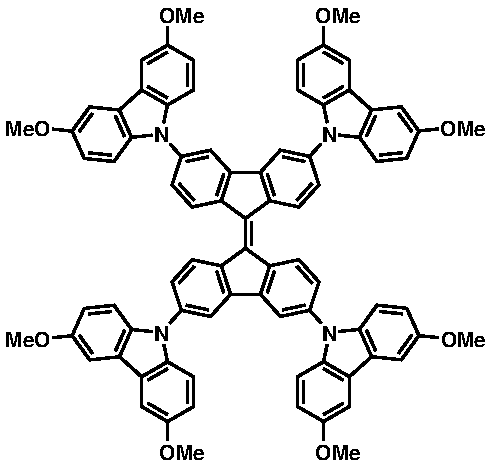
\includegraphics[scale=0.8]{molecules/tae4.pdf}
				\subcaption{\gls{tae4}}\label{fig:tae-molecules-tae4}
			\end{subfigure}
			\mycaption[Chemical structures of HTM utilised for bottom cathode solar cells.]{}\label{fig:tae-molecules}
		}
	}
\end{figure}

\paragraph{Design of the Experiment}
Differently from our previous report on \gls{tae1} \cite{Cabau2015a}, we decided to avoid the mesoporous titania layer in order to decrease the complexity of the stack.
In order to compare different materials for the selective contact layer, we decided to avoid any modification to the layers underlying the absorber one in the solar cell stack, as these could heavily affect the perovskite morphology \cite{Tao2017}.
%The variation of the upper contact (\textsl{i.e.} the \gls{htm} in bottom cathode solar cells) guarantees that the observed differences will not be due to a different perovskite structure, whose crystallization has been reported to be sensible to the underlying contact 
Additionally, the \gls{htm} under comparison have been deposited under as similar as possible conditions (partially hindered by a different solubility), employing the same additives and thicknesses.
For reducing the possible differences in \gls{dos} width, the chosen \gls{htm} have all very similar chemical structures.


\paragraph{Author contributions}
The devices have been fabricated by me under the supervision of Dr.\ Nuria F.\ Montcada and Prof.\ Emilio J.\ Palomares Gil (fabrication described in \cpagerefrange{methods_bottom}{methods_bottom_end}).
The current\hyp{}voltage sweeps characterization was performed by me and NFM.
The transient electronic characterization was performed and analysed by me using equipment built by Dr.\ Javier Pérez Hernández.
The electrochemical and optical characterization of the molecules was performed by NFM, Dr.\ Lydia Cabau, Dr.\ Agustín Molina Ontoria, and Dr.\ Inés García\hyp{}Benito.
Molecular simulations have been performed by Prof.\ Anton Vidal\hyp{}Ferran.
Dr.\ Agustín Molina Ontoria and Prof. Nazario Martín designed \gls{tae1}, \gls{tae3}, and \gls{tae4} molecules.
The synthesis of these has been carried on by Dr.\ Inés García\hyp{}Benito and reported in her PhD thesis \cite{Garcia-Benito2017} (there, \gls{tae3} is labelled as BF-1, and \gls{tae4} as BF-2) and in \cite{Gelmetti2019}.
\Gls{kpfm} measurements has been performed by Dr.\ Ana Pérez-Rodríguez, Dr.\ Esther Barrena, and Prof.\ Carmen Ocal at ICMAB-CSIC, UAB, Barcelona.


% Belisle2016 In the ionic accumulation case (Figure 3b), these variations in the HTM are accommodated by a vacuum-level shift (drawn here as enabled by the accumulation of positive charge such as iodide vacancies theorized to exist in these materials(43)) at the interface, screening the electric field across the perovskite and leaving carrier densities, and therefore recombination, independent of the HTM.
%

%
%
\section{Molecular Characterization}

%\afterpage{
	\begin{table}%[h]	% longtables cannot stay inside a float, otherwise they will not break
	\begin{xltabular}[c]{1.05\linewidth}{@{} >{\hsize=1.5\hsize}Y | >{\hsize=1.5\hsize}Y >{\hsize=0.7\hsize}Y >{\hsize=0.7\hsize}Y >{\hsize=0.9\hsize}Y >{\hsize=0.9\hsize}Y >{\hsize=0.9\hsize}Y >{\hsize=0.9\hsize}Y Y @{}}
		% multirow does not get the correct number of rows with tabularx
		% mycaption does not work inside xltabular
		\caption[Molecular properties of tested HTM.]{\textbf{Molecular properties of tested HTM.}
			The values for \gls{spiro} and for \gls{tae1} were taken from our previous publication \cite{Cabau2015a}.
			$E^{\mathrm{abs}}_|onset|$ is the direct optical band gap obtained \textsl{via} Tauc plot.
			$E^{\mathrm{pl}}_|max|$ indicates the energy of the emission peak obtained exciting at \SI{550}{\nm} a solution of the molecule in \gls{thf}.
			$E^{\mathrm{exp}}_|HOMO|$ is obtained from the cyclic voltammetry of the molecules dissolved in \gls{dcm} and using ferrocene as reference.
			$E^{\mathrm{exp}}_|LUMO|$ is obtained adding the direct optical band gap $E^{\mathrm{abs}}_|onset|$ to $E^{\mathrm{exp}}_|HOMO|$ except for \gls{tae1} where the value from \cite{Cabau2015a} has been taken.
			$E^{\mathrm{sim}}_|HOMO|$ and $E^{\mathrm{sim}}_|LUMO|$ have been obtained via a \gls{dft} simulation.
			$E^{\mathrm{sim,abs}}_|onset|$ is the direct optical band gap obtained \textsl{via} Tauc plot of the absorbance simulated with time-dependent \gls{dft}.
		}\label{table:tae_molecular}\\[\belowcaptionskip]
%		\rule[-1ex]{0pt}{3ex} \\
%		\multirow{2}{*}{\small\gls{htm}} & \small$\mu_|h|$ & \small$E^{\mathrm{abs}}_|onset|$ & \small$E^{\mathrm{pl}}_|max|$ & \small$E_|g|$ & \small$E_|ox|$ & \small$E^{\mathrm{exp}}_|HOMO|$ & \small$E^{\mathrm{exp}}_|LUMO|$ & \small$E^{\mathrm{sim}}_|HOMO|$ & \small$E^{\mathrm{sim}}_|LUMO|$\\ 
				\multirow{2}{*}{\small\gls{htm}} & \small$\mu_|h|$ & \small$E^{\mathrm{abs}}_|onset|$ & \small$E^{\mathrm{pl}}_|max|$ & \small$E^{\mathrm{exp}}_|HOMO|$ & \small$E^{\mathrm{exp}}_|LUMO|$ & \small$E^{\mathrm{sim}}_|HOMO|$ & \small$E^{\mathrm{sim}}_|LUMO|$ & \small$E^{\mathrm{sim,abs}}_|onset|$ \\ 
		\rule[-1ex]{0pt}{2.5ex}
%		   & \footnotesize\si{\square\cm\per\V\per\s} & \footnotesize\si{nm} & \footnotesize\si{nm} & \footnotesize\si{\eV} & \footnotesize\si{\V} & \footnotesize\si{\eV} & \footnotesize\si{\eV} & \footnotesize\si{\eV} & \footnotesize\si{\eV} \\[1mm]
		   		   & \footnotesize\si{\square\cm\per\V\per\s} & \footnotesize\si{\eV} & \footnotesize\si{\eV} & \footnotesize\si{\eV} & \footnotesize\si{\eV} & \footnotesize\si{\eV} & \footnotesize\si{\eV} & \footnotesize\si{\eV} \\[1mm]
		\hline
		\endfirsthead
		\multicolumn{2}{@{}l}{\ldots \small continues}\\
		\hline
%		\small\gls{htm} & \small$\mu_|h|$ & \small$E^{\mathrm{abs}}_|onset|$ & \small$E^{\mathrm{pl}}_|max|$ & \small$E_|g|$ & \small$E_|ox|$ & \small$E^{\mathrm{exp}}_|HOMO|$ & \small$E^{\mathrm{exp}}_|LUMO|$ & \small$E^{\mathrm{sim}}_|HOMO|$ & \small$E^{\mathrm{sim}}_|LUMO|$\\ 
				\small\gls{htm} & \small$\mu_|h|$ & \small$E^{\mathrm{abs}}_|onset|$ & \small$E^{\mathrm{pl}}_|max|$ & \small$E^{\mathrm{exp}}_|HOMO|$ & \small$E^{\mathrm{exp}}_|LUMO|$ & \small$E^{\mathrm{sim}}_|HOMO|$ & \small$E^{\mathrm{sim}}_|LUMO|$ & \small$E^{\mathrm{sim,abs}}_|onset|$\\ 
		\hline
		\endhead
		\hline
		\multicolumn{9}{r@{}}{\small continues\ldots}\\
		\endfoot
		\hline
		\endlastfoot
		\rule[-1ex]{0pt}{3ex}
%		spiro\hyp{}OMeTAD 	& \num{2.6E-4} 	& \num{}	& \num{}	& \num{3.01}	& \num{-5.10}	& \num{-2.09}	& \num{}	& \num{}  \\
%		TAE-1				& \num{5.9E-5} 	& \num{}	& \num{}	& \num{2.58}	& \num{-5.32}	& \num{-2.74}	& \num{-5.61}	& \num{-0.54}  \\
%		TAE-3 				& \num{8E-4} 	& \num{1.836}	& \num{1.722}	& \num{1.84}	& \num{-5.00}	& \num{-3.16}	& \num{-5.54}	& \num{-1.77}  \\
%		TAE-4 				& \num{7E-4} 	& \num{1.969}	& \num{1.771}	& \num{1.97}	& \num{-5.53}	& \num{-3.56}	& \num{-6.14}	& \num{-2.27} \\
		spiro-OMeTAD 		& \num{2.6E-4} 	& 				& 					& \num{-5.10}	& \num{-2.09}	& 				&  				& \\
		TAE-1				& \num{5.9E-5} 	& \num{2.813}	& 					& \num{-5.32}	& \num{-2.74}	& \num{-5.61}	& \num{-0.54}	& \num{3.04} \\
		TAE-3 				& \num{8E-4} 	& \num{1.836}	& \num{1.722}		& \num{-5.00}	& \num{-3.16}	& \num{-5.54}	& \num{-1.77}	& \num{2.02} \\
		TAE-4 				& \num{7E-4} 	& \num{1.969}	& \num{1.771}		& \num{-5.53}	& \num{-3.56}	& \num{-6.14}	& \num{-2.27}	& \num{2.20} \\
	\end{xltabular}
\end{table}

\paragraph{HOMO from cyclic voltammetry}
The oxidation potential of each \gls{htm} has been measured \textsl{via} cyclic voltammetry in solution.
Then the energy of \gls{homo}, reported in \cref{table:tae_molecular}, has been obtained from the oxidation potential \textsl{via} the empirical relationship reported in \authoryear{DAndrade2005}.

\begin{SCfigure}
	\centering
	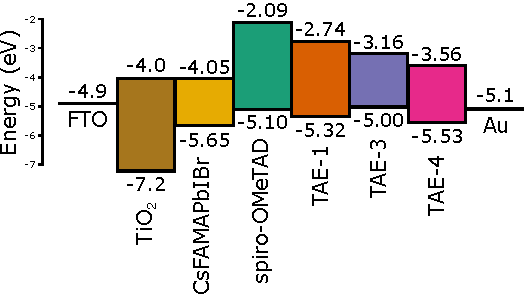
\includegraphics[width=0.7\textwidth]{energy_levels/energy_levels.pdf}
	\mycaption[Representation of HOMO and LUMO energies for the materials composing the studied cells.]{
		The \gls{homo} energy has been estimated from the oxidation potential obtained \textsl{via} cyclic voltammetry and the direct optical band gap from a Tauc plot, as described in the text.
	}\label{fig:tae-energy_levels}
\end{SCfigure}

\paragraph{Direct optical band gap}
We extracted the direct band gap value from the direct Tauc plot of the absorbance onset \cite{WikipediaTauc}, an easy technique developed for amorphous semiconductors \cite{Stenzel2005} with delocalized orbitals but often employed also for small molecules.
A closely related value can be obtained from the photoluminescence peak maximum, which is also reported in \cref{table:tae_molecular}.
The shape of the absorbance onset (Urbach tail) of an \gls{htm}, additionally to provide information on its optical band gap, can reveal the presence of mid-gap states which would favour the surface recombination \cite{Tvingstedt2017}.

\paragraph{Simulated energy levels}
As can be seen in \cref{table:tae_molecular}, the \gls{dft} simulated $E^{\mathrm{sim}}_|HOMO|$ manages to reproduce the trend of the experimental $E^{\mathrm{exp}}_|HOMO|$, being the \gls{tae4} the deepest and \gls{tae3} the shallowest.
Contrariwise, the simulated $E^{\mathrm{sim}}_|LUMO|$ values are rather distant from the experimental $E^{\mathrm{exp}}_|LUMO|$ ones, even if the trend is correctly reproduced.
This can be understood considering that the $E^{\mathrm{sim}}_|LUMO|$ is simulated on top of the non\hyp{}excited molecule, which is the molecule with a fully occupied \gls{homo} level.
This situation does not properly describe the final point of an excitation transition, where the \gls{homo} is not full as one electron have been promoted to \gls{lumo}.
The energetic difference between the two described configurations is an electron\hyp{}hole interaction energy, which is the origin of the exciton binding energy described in \cpageref{intro_geminate}.
The experimental direct optical band gap \small$E^{\mathrm{abs}}_|onset|$ can be fairly compared with the value $E^{\mathrm{sim,abs}}_|onset|$ obtained from the onset of a absorption spectra simulated with time\hyp{}dependent \gls{dft}.

\paragraph{Mobility}


\section{Devices Morphological Characterization}

\paragraph{X--Ray diffraction}


\section{Devices Performances}

\paragraph{}

\section{Charge Extraction}

\paragraph{}

\section{Transient Life-Time}

\paragraph{}

\section{Workfunction of Stacked Materials}

\paragraph{}
Further characterization of the workfunction of the \gls{htm} surface when layered on top of \gls{fto} or \ch{TiO2} or \gls{csfamapbibr} has been performed using \gls{kpfm}.
The measured \gls{cpd} allowed us to study the impact the underlying perovskite layer can have on the \gls{htm} material.
These measurements have been discussed in Dr.\ Ana Pérez-Rodríguez PhD thesis \cite{Perez-Rodriguez2018}.

%"the often-questionable validity of vacuum level alignment, the importance of interface dipoles, and band bending as the result of interface formation" \cite{Schulz2019}